\documentclass{article}

\usepackage{fullpage}
\usepackage{siunitx}
\usepackage{graphicx}
\usepackage{hyperref}
\hypersetup{colorlinks=true, linkcolor=blue}
\usepackage{wrapfig}

%\usepackage{titlesec}
%\newcommand{\sectionbreak}{\clearpage}
%\let\stdsection\section
%\renewcommand\section{\newpage\stdsection}

\setlength{\parindent}{0pt}
\setlength{\parskip}{2ex plus 1ex minus 1ex}

%\usepackage{feffitplots}        % big, icky layouts for the grids of plots




\begin{document}

\appendix


\section{Background}


The
\href{http://leonardo.phys.washington.edu/feff/wiki/static/i/o/r/IORDER_326d.html}%
{\textsc{feff} document} tells us this about the \texttt{IORDER} parameter
(links and some formatting added by me):

\begin{quote}
  Order of the approximation used in module \texttt{GENFMT}.
  \textsc{feff} uses order 2 by default, which is correct to terms of
  order $(pR)^{-2}$ and corresponds to $6\times6$ scattering matrices
  in the Rehr-Albers formalism.  Single scattering is calculated
  exactly to this order.  The $6\times6$ approximation is accurate to
  within a few percent in every case we have tried (that is, higher
  order doesn’t change the result more than a few percent). However
  $M_{IV}$ shells and higher shells may require increased iorder for
  coupling the matrix elements.  Changing the default values requires
  some familiarity with the Rehr-Albers paper and the structure of the
  module \texttt{GENFMT}.  To do so, follow the instructions in the
  feff source code in subroutine
  \href{https://github.com/xraypy/feff85exafs/blob/master/src/GENFMT/setlam.f}%
  {\texttt{setlam}}.  The key \texttt{iord} is passed to
  \texttt{setlam} for processing.  You may need to change
  \href{https://github.com/xraypy/feff85exafs/blob/master/src/HEADERS/dim.h#L37}%
  {the code parameter \texttt{lamtot}} if you want to do higher order
  calculations.  For details of the algorithm used by \texttt{GENFMT},
  see \href{http://dx.doi.org/10.1103/PhysRevB.41.8139}%
  {the paper by J.J. Rehr and R.C. Albers}. For the $M_{IV}$ and
  higher edges, you may receive an error message like: Lambda array
  overfilled. In that case the calculations should be repeated with
  \texttt{IORDER -70202} ($10\times10$ matrices).
\end{quote}

To test the effect of changing the \texttt{iord} parameter on EXAFS
analysis, I compiled up a copy of the \textsc{genfmt} program with 
\href{https://github.com/xraypy/feff85exafs/blob/master/src/HEADERS/dim.h}%
{\texttt{/src/HEADERS/dim.h}} modified with \texttt{lamtot=35},
\texttt{mtot=6}, and \texttt{ntot=4}.

\textit{Caveat:} I selected those values based on my understanding of
\href{https://github.com/xraypy/feff85exafs/blob/master/src/GENFMT/setlam.f}%
{\texttt{setlam.f}}.  \textsc{genfmt} ran to completion without
complaint, so I am hopeful that that was done correctly.

For each material (see the SCF tests document for descriptions of the
materials), I computed \textsc{feff} with self-consistency and the
self-consistency radius set to the \textit{second shortest} value used
in the SCF tests.  For example, for FeS$_2$, the radius was set to
3.6\,\AA\ and, for BaZrO$_3$, the radius was set to 4\,\AA.  I then
ran calculations with the \texttt{iord} parameter set to 1, 2, 3, 4,
and 10.
\href{https://github.com/xraypy/feff85exafs/blob/master/src/GENFMT/setlam.f#L60}%
{The code} identifies 10 as triggering the ``cute'' algorithm, which
treats collinear paths differently from other multiple scattering
paths.

Changes to the \texttt{iord} parameter should only effect multiple
scattering paths.  Single scattering paths are calculated without that
approximation.  This is easily tested.  Running a sequence of first
shell fits with different values if \texttt{iord} does, in fact,
result in identical fit results.  For example, here are the results
for first shell fits to FeS$_2$:

\begin{wrapfigure}{r}{0.35\textwidth}
  \vspace{-40pt}
  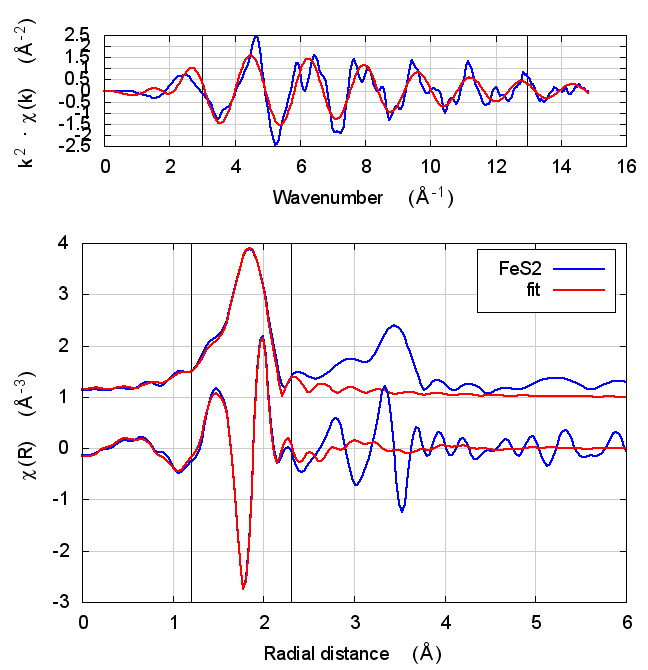
\includegraphics[width=0.35\textwidth]{FeS2/iorder/fit_iorder_02_1st.png}
\end{wrapfigure}
\small
\input{FeS2/iorder/FeS2_1st.tex}
\normalsize

The fits are not plotted here.  In all cases, the fit quality is
comparable to what is shown in the SCF test document.  The small
differences between the different \texttt{iord} values is hard to see
in the plot.  Thus, only the tables are presented here.

\section{Copper}

\small
\input{Copper/iorder/Copper.tex}
\normalsize

\section{NiO}

\small
\input{NiO/iorder/NiO.tex}
\normalsize

\section{FeS$_2$}

\small
\input{FeS2/iorder/FeS2.tex}
\normalsize

\section{UO$_2$}

\scriptsize
\input{UO2/iorder/UO2.tex}
\normalsize

\section{BaZrO$_3$}

\scriptsize
\input{BaZrO3/iorder/BaZrO3.tex}
\normalsize

\section{bromoadamantane}

\small
\input{bromoadamantane/iorder/bromoadamantane.tex}
\normalsize

\section{uranyl}

\small
\input{uranyl/iorder/uranyl.tex}
\normalsize

\section{Discussion}

\begin{enumerate}
\item A couple of the materials pretty much as one might expect.
  NiO, Bromoadamantane, and BaZrO$_3$ show a significant drop in
  $\chi_\nu^2$ between \texttt{iord} of 1 and 2, while not showing a
  statistcially significant change in any of the fitting parameters.
\item A few materials -- Copper, FeS$_2$, and uranyl -- actually show
  somewhat better $\chi_\nu^2$ for \texttt{iord} of 1.  I think this
  tells us that at \texttt{iord} of 1, the calculation is not
  converged and that the effect of this on the EXAFS analysis is
  ill-determined.  I think it would be a mistake to claim something
  like ``fitting is better in some cases with \texttt{iord}=1.''
  Rather, this variability is telling us that \texttt{iord}=1 is a
  mistake.
\item In most cases, there is very little change in $\chi_\nu^2$ for
  \texttt{iord}\,$\ge2$.  While there is some variability among the
  larger \texttt{iord} results for some materials (NiO, for example,
  varied by a bit more than 1\%), it seems that the default of
  \texttt{iord}\,$=2$ is well justified.
\item Perhaps this exercise could be used to approximate the
  systematic uncertainty contributed by the MS theory to the EXAFS
  analysis....
\end{enumerate}


\end{document}

%%% Local Variables:
%%% mode: latex
%%% TeX-master: t
%%% TeX-parse-self: t
%%% TeX-auto-save: t
%%% TeX-auto-untabify: t
%%% TeX-PDF-mode: t
%%% End:
